% 保留原始面板、实拍、示例与全部连线；仅以 TikZ 覆盖说明标签。
\begin{tikzpicture}
\node[anchor=south west,inner sep=0] (im) at (0,0) {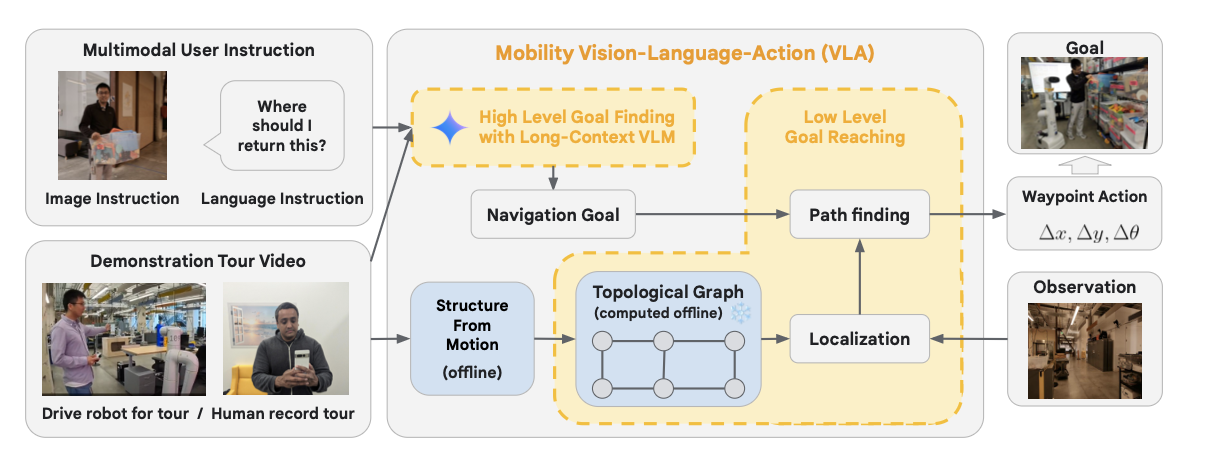
\includegraphics[width=\linewidth]{figures/mobility.png}};
\begin{scope}[x={(im.south east)},y={(im.north west)}]
\fill[white] (0.047855,0.865217) rectangle (0.283828,0.915217);
\node[align=center,inner sep=0pt,font=\fontsize{8.5}{9.5}\selectfont,text width=0.235974\linewidth,rotate=0] at (0.165842,0.890217) {多模态用户指令};
\fill[white] (0.400990,0.854348) rectangle (0.754950,0.915217);
\node[align=center,inner sep=0pt,font=\fontsize{9}{10}\selectfont,text width=0.353960\linewidth,rotate=0] at (0.577970,0.884783) {Mobility 视觉语言动作模型};
\fill[white] (0.858911,0.873913) rectangle (0.936469,0.921739);
\node[align=center,inner sep=0pt,font=\fontsize{8.5}{9.5}\selectfont,text width=0.077558\linewidth,rotate=0] at (0.897690,0.897826) {目标};
\fill[white] (0.191419,0.652174) rectangle (0.276403,0.793478);
\node[align=center,inner sep=0pt,font=\fontsize{8}{9}\selectfont,text width=0.084983\linewidth,rotate=0] at (0.233911,0.722826) {我该把这个\\放回哪里？};
\fill[white] (0.035479,0.539130) rectangle (0.165017,0.584783);
\node[align=center,inner sep=0pt,font=\fontsize{8}{9}\selectfont,text width=0.129538\linewidth,rotate=0] at (0.100248,0.561957) {图像指令};
\fill[white] (0.163366,0.532609) rectangle (0.305281,0.589130);
\node[align=center,inner sep=0pt,font=\fontsize{8}{9}\selectfont,text width=0.127063\linewidth,rotate=0] at (0.241749,0.560870) {语言指令};
\fill[white] (0.050330,0.400000) rectangle (0.274752,0.452174);
\node[align=center,inner sep=0pt,font=\fontsize{8.5}{9.5}\selectfont,text width=0.224422\linewidth,rotate=0] at (0.162541,0.426087) {示范巡视视频};
\fill[white] (0.027228,0.063043) rectangle (0.303630,0.128261);
\node[align=center,inner sep=0pt,font=\fontsize{7.8}{8.8}\selectfont,text width=0.276403\linewidth,rotate=0] at (0.165429,0.095652) {机器人巡视／人工录制巡视};
\fill[white] (0.387789,0.676087) rectangle (0.564356,0.765217);
\node[align=center,inner sep=0pt,font=\fontsize{6.8}{7.8}\selectfont,text width=0.176568\linewidth,rotate=0] at (0.476073,0.720652) {用长上下文视觉语言模型\\寻找高层目标};
\fill[white] (0.400990,0.510870) rectangle (0.512376,0.560870);
\node[align=center,inner sep=0pt,font=\fontsize{8}{9}\selectfont,text width=0.111386\linewidth,rotate=0] at (0.456683,0.535870) {导航目标};
\fill[white] (0.351485,0.158696) rectangle (0.428218,0.363043);
\node[align=center,inner sep=0pt,font=\fontsize{8}{9}\selectfont,text width=0.076733\linewidth,rotate=0] at (0.389851,0.260870) {运动恢复\\结构\\（离线）};
\fill[white] (0.485149,0.291304) rectangle (0.623000,0.384783);
\node[align=center,inner sep=0pt,font=\fontsize{8}{9}\selectfont,text width=0.127888\linewidth,rotate=0] at (0.549092,0.338043) {拓扑图\\（离线计算）};
\fill[white] (0.643000,0.663043) rectangle (0.780000,0.763043);
\node[align=center,inner sep=0pt,font=\fontsize{8}{9}\selectfont,text width=0.125413\linewidth,rotate=0] at (0.712871,0.713043) {底层目标\\到达};
\fill[white] (0.660891,0.506522) rectangle (0.759901,0.563043);
\node[align=center,inner sep=0pt,font=\fontsize{8}{9}\selectfont,text width=0.099010\linewidth,rotate=0] at (0.710396,0.534783) {路径搜索};
\fill[white] (0.655116,0.234783) rectangle (0.761551,0.291304);
\node[align=center,inner sep=0pt,font=\fontsize{8}{9}\selectfont,text width=0.106436\linewidth,rotate=0] at (0.708333,0.263043) {定位};
\fill[white] (0.841584,0.536957) rectangle (0.958746,0.600000);
\node[align=center,inner sep=0pt,font=\fontsize{7.5}{8.5}\selectfont,text width=0.117162\linewidth,rotate=0] at (0.900165,0.568478) {航路点动作};
\fill[white] (0.852310,0.350000) rectangle (0.947195,0.400000);
\node[align=center,inner sep=0pt,font=\fontsize{8}{9}\selectfont,text width=0.094884\linewidth,rotate=0] at (0.899752,0.375000) {观测};
\end{scope}
\end{tikzpicture}
